Одной из поставленных на текущий семестр задач было изучение технологии юнит-тестирования в инструментарии Qt и внедрение тестирования. Внедрение производилось в модуль, сканирующий медиа-файлы.

Модульное тестирование, или юнит-тестирование --- процесс в программировании, позволяющий проверить на корректность отдельные модули исходного кода программы.

Идея состоит в том, чтобы писать тесты для каждой нетривиальной функции или метода. Это позволяет достаточно быстро проверить, не привело ли очередное изменение кода к появлению ошибок в уже оттестированных местах программы, а также облегчает обнаружение и устранение таких ошибок.

Для начала необходимо было понять, как работает юнит-тестирование в инструментарии Qt. Для этого была написана простейшая программа, возводящая входное число во вторую и третью степень. В программе имелся класс с двумя методами, каждый из которых реализовывал соответствующую функцию, а для класса, реализующего тестирование, необходимо было создать подпроект.

Для того, чтобы составить набор тестов, инструментарий Qt позволяет использовать специальную <<таблицу>>, в которой распределены столбцы с входными и выходными данными, и каждый новый тест заносится как строка. Далее, с помощью макроса QFETCH данные <<таблицы>> переносятся непосредственно в тестирующую функцию, которая сравнивает выходной результат с ожидаемым.

Входные данные для тестирования представлены в таблице~\ref{tab:1}.

\begin{table}[h]
\caption{ Входные данные для тестирования }
\label{tab:1}
\begin{center}
\begin{tabularx}{\linewidth}{|X|X|X|X|X|X|}
\hline
\multicolumn{6}{|c|}{Данные для функции возведения во вторую степень} \\
\hline
Data & 1 & -1 & 4 & 0 & -10 \\
\hline
Result & 1 & 1 & 16 & 0 & 100 \\
\hline
\multicolumn{6}{|c|}{Данные для функции возведения в третью степень} \\
\hline
Data & 1 & -1 & 4 & 0 & -10 \\
\hline
Result & 1 & -1 & 64 & 0 & -1000 \\
\hline
\end{tabularx}
\end{center}
\end{table}

Выходной результат сравнивался с ожидаемым с помощью макроса QCOMPARE. Далее необходимо было подключить тестовый подпроект к основному проекту, чтобы иметь возможность использовать классы и методы главного проекта, и использовать макроc QTEST\_APPLESS\_MAIN для запуска тестирования, результат которого выводился непосредственно в среду разработки.
 
После исследования юнит-тестирования и ознакомления с его использованием в инструментарии Qt, началась имплементация тестирования в модуль, сканирующий медиа-файлы.

В качестве входных данных в таблицу подавалось имя файла, а на выходе ожидался массив строк с корректными метаданными (табл.~\ref{tab:2},~\ref{tab:3},~\ref{tab:4}).

\begin{table}[h!]
\caption{ Входные данные для функции чтения тегов id3 }
\label{tab:2}
\begin{center}
\begin{tabularx}{\linewidth}{|X|X|X|X|X|}
\hline
Path & Title & Artist & Album & Date \\
\hline
No Man's Ship Master.mp3 & No-Man's Ship & Cult Of Violence & No-Man's Ship & 2015 \\
\hline
Dig.mp3 & Dig & Mudvayne & L.D. 50 & 2000 \\
\hline
\end{tabularx}
\end{center}
\end{table}

\begin{table}[h!]
\caption{ Входные данные для функции чтения тегов jfif }
\label{tab:3}
\begin{center}
\begin{tabularx}{\linewidth}{|X|X|X|X|X|X|X|}
\hline
Path & Bits per pixels & Width & Height & Pixel Density & X resolution & Y resolution \\
\hline
doctor-who-19033.jpg & 8 & 1050 & 1680 & No units & 72 & 72 \\
\hline
pic\_jpg.jpg & 8 & 1001 & 1419 & No units & 300 & 300 \\
\hline
\end{tabularx}
\end{center}
\end{table}

\begin{table}[h!]
\caption{ Входные данные для функции чтения тегов riff }
\label{tab:4}
\begin{center}
\begin{tabularx}{\linewidth}{|X|X|X|X|X|}
\hline
Path & Width & Height & Channels & Sample rate \\
\hline
Gintama.avi & 640 & 480 & 2 & 48000 \\
\hline
\end{tabularx}
\end{center}
\end{table}

Результат тестирования методов представлены на рисунках~\ref{Screenshot_2:Screenshot_2} и~\ref{Screenshot_1:Screenshot_1}.

\begin{figure}[h!]
\center{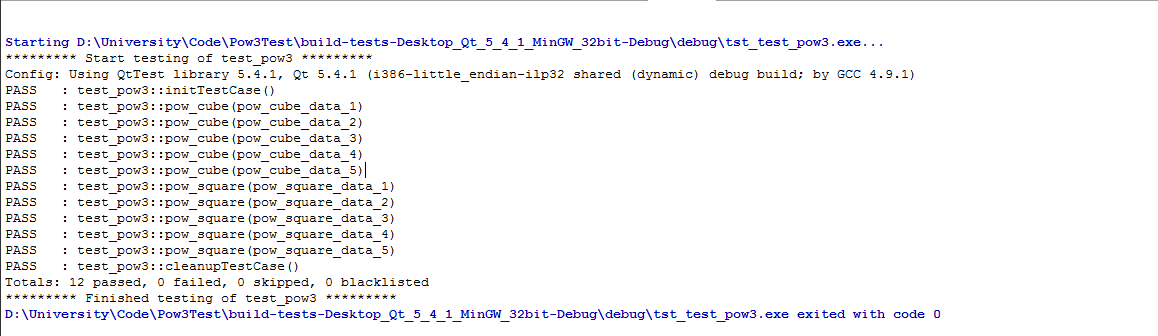
\includegraphics[width=0.9\linewidth]{Screenshot_1}}
\caption{ Результат успешного тестирования методов pow\_cube и pow\_square }
\label{Screenshot_1:Screenshot_1}
\end{figure} 

\begin{figure}[h!]
\center{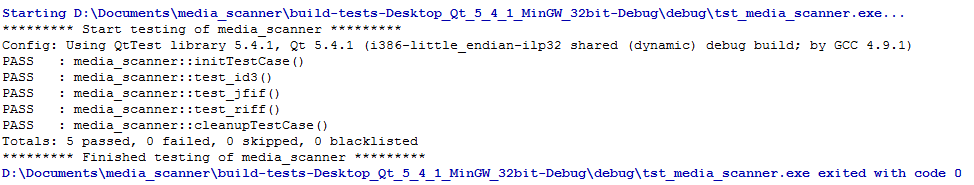
\includegraphics[width=0.9\linewidth]{Screenshot_2}}
\caption{ Результат успешного тестирования методов }
\label{Screenshot_2:Screenshot_2}
\end{figure} 

\clearpage






